\sectioncounter{43}

\section{双曲线及其方程}

\subsection{知识梳理}
设两个定点 $F_1$, $F_2$ 之间的距离为 $2c>0$, 动点 $P$ 满足 
\[\big||PF_1|-|PF_2|\big|= 2a<2c,\]
其中 $a$ 为定值, 则点 $P$ 运动时形成的轨迹 $C$ 称为双曲线, $F_1$, $F_2$ 为双曲线 $C$ 的两个焦点, $2c$ 为焦距而 $c$ 为半焦距. 以直线 $F_1F_2$ 为 $x$ 轴, 线段 $F_1F_2$ 中垂线为 $y$ 轴, 
建立平面直角坐标系 (图 \ref{fig-190323-2110}), 则 $F_1(-c,0)$, $F_2(c,0)$ 分别为双曲线的左焦点、右焦点. 图中双曲线分为两部分, 分别称为左支和右支.

\begin{figure}[hb]
    \centering
    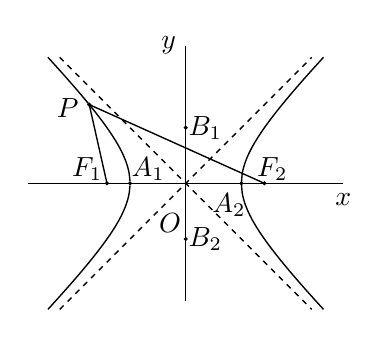
\begin{tikzpicture}[scale=0.5]
      \draw[\myaxisarrow] (-4,0) -- (4,0) 
        node[below] {$x$} coordinate(x axis);
      \draw[\myaxisarrow] (0,-3) -- (0,3.5) 
        node[left] {$y$} coordinate(y axis);
      \draw[line width=0.5pt,smooth,samples=100,domain=1.414214:3.5] 
        plot(\x,{sqrt((\x)^2-2)});
      \draw[line width=0.5pt,smooth,samples=100,domain=1.414214:3.5] 
        plot(\x,-{sqrt((\x)^2-2)});
      \draw[line width=0.5pt,smooth,samples=100,domain=-3.5:-1.414215] 
        plot(\x,{sqrt((\x)^2-2)});
      \draw[line width=0.5pt,smooth,samples=100,domain=-3.5:-1.414215] 
        plot(\x,-{sqrt((\x)^2-2)});
      \draw [line width=0.5pt,dash pattern=on 2pt off 2pt] (-3.2,-3.2)-- (3.2,3.2);
      \draw [line width=0.5pt,dash pattern=on 2pt off 2pt] (-3.2,3.2)-- (3.2,-3.2);
      \draw [line width=0.5pt] (-2.,0.)-- (-2.45,2);
      \draw [line width=0.5pt] (-2.45,2)-- (2.,0.);
      
      \draw [fill=black] (-2.,0.) circle (1pt);
      \draw[color=black] (-2.5,0.37) node {$F_1$};
      \draw [fill=black] (2.,0.) circle (1pt);
      \draw[color=black] (2.2,0.37) node {$F_2$};
      \draw [fill=black] (-1.4142,0.) circle (1pt);
      \draw[color=black] (-0.95,0.37) node {$A_1$};
      \draw [fill=black] (1.4142,0.) circle (1pt);
      \draw[color=black] (1.1,-0.55) node {$A_2$};
      \draw [fill=black] (0,1.414) circle (1pt);
      \draw[color=black] (0.5,1.414) node {$B_1$};
      \draw [fill=black] (0,-1.414) circle (1pt);
      \draw[color=black] (0.5,-1.414) node {$B_2$};
      \draw [fill=black] (-2.45,2) circle (1pt);
      \draw[color=black] (-3,1.9) node {$P$};
      \draw (-0.4,-1) node {$O$};
    \end{tikzpicture}
    \caption{}\label{fig-190323-2110}
\end{figure}

再设 $P(x,y)$, 则由两点之间距离公式, 上面的等式化为
\[|\sqrt{(x+c)^2+y^2}-\sqrt{(x-c)^2+y^2}|= 2a,\]
进一步可以简化为
\[\frac{x^2}{a^2}-\frac{y^2}{c^2-a^2}=1.\]
令 $c^2-a^2=b^2$ ($b>0$), 则得双曲线的标准方程
\[C\colon \frac{x^2}{a^2}-\frac{y^2}{b^2}=1.\]
注意, 上式表示中心为原点、焦点在 $x$ 轴上 (左右开口) 的双曲线的标准方程, 而中心为原点、焦点在 $y$ 轴上 (上下开口) 的双曲线的标准方程形如
\[C'\colon \frac{y^2}{a^2}-\frac{x^2}{b^2}=1.\]
以下只分析前一种双曲线, 对后一种也有类似的结论.

由 $c^2-a^2=b^2$ 知 $c^2=a^2+b^2$, 即 $c$ 值最大. 定义 $e=\dfrac{c}a$ 为双曲线的离心率, 则 $e\in(1,+\infty)$.
\mymarginpar{$e$ 的大小可以刻画双曲线的形状: $e$ 越接近 $1$, 双曲线开口越小; $e$ 越接大, 双曲线开口越大.}
双曲线 $C$ 的方程表明其为轴对称图形和中心对称图形, 且对称轴为 $x$ 轴和 $y$ 轴, 对称中心为原点, 故原点也称为 $C$ 的中心. 双曲线 $C$ 与 $x$ 轴交于 $A_1(-a,0)$ (左顶点), $A_2(a,0)$ (右顶点), 与 $y$ 轴无交点,但仍类似椭圆取 $B_1(0,b)$, $B_2(0,-b)$. 称线段 $A_1A_2$ 为双曲线 $C$ 的实轴, $B_1B_2$ 为其虚轴, 而 $a$, $b$ 分别为实半轴长和虚半轴长. 此外还有 $|A_1B_1|=c$.

双曲线有两条渐近线.
\mymarginpar{初中学过的反比例函数 $y=\dfrac1x$ 的图形也为双曲线, 中心为原点, 对称轴为 $y= \pm x$, 渐近线为坐标轴.}%
对双曲线 $C\colon \dfrac{x^2}{a^2}-\dfrac{y^2}{b^2}=1$, 求其渐近线时, 只需令等号右边的常数项为 $0$, 再移项开方可得渐近线方程: $y=\pm\dfrac{b}ax$. 反之, 若已知双曲线 $C$ 的渐近线方程为 $y=\pm\dfrac{b}ax$, 则可设
\[C\colon \frac{x^2}{a^2}-\frac{y^2}{b^2}=m\ (m\neq0).\]


\lianxi
\begin{exercise}
    设双曲线 $C\colon x^2- \dfrac{y^2}{9}=1$ 的左焦点、右焦点分别为 $F_1$,$F_2$, 点 $P$ 在 $C$ 上且 $|PF_1|= 3$, 求 $|PF_2|$ 的值.
\end{exercise}
\beginsolution
    由双曲线的定义,
    \[\bigl||PF_1|- |PF_2|\bigr|= 2\cdot 1,\quad
    |PF_2|= 1,5.\]
\endsolution

\begin{exercise}
    若双曲线 $C\colon x^2 -\dfrac{y^2}m =1$ 的实轴长是虚轴长的 $2$ 倍, 求 $m$ 的值.
\end{exercise}
\beginsolution
    由题意, $1= 2\cdot \sqrt2$, $m=\dfrac14$.
\endsolution

\begin{exercise}
    设双曲线 $C$ 的中心为原点, 焦点在坐标轴上, 离心率 $e=\sqrt3$, 且过点 $A(1,1)$, 求双曲线 $C$ 的标准方程.
\end{exercise}
\beginsolution
    设实半轴长为 $a$, 虚半轴长为 $b$, 半焦距为 $c$, 则 $e= \dfrac{c}a= \sqrt3$. 结合 $c^2= a^2+b^2$ 可设
    \[c=\sqrt3k,\ a=k,\ b=\sqrt2k,\quad k>0.\]

    若焦点在 $x$ 轴上, 则双曲线 $C$ 的方程为 $\dfrac{x^2}{k^2}- \dfrac{y^2}{2k^2}= 1$. 将 $A(1,1)$ 代入知, $k^2= \dfrac12$, 所求方程为 $2x^2-y^2= 1$.

    若焦点在 $y$ 轴上, 同理可知, 双曲线 $C$ 的方程为 $2y^2- x^2= 1$.
\endsolution

\begin{exercise}
    求经过点 $A(-\sqrt3, 6)$, 且渐近线为 $y=\pm 3x$ 的双曲线 $C$的方程.
\end{exercise}
\beginsolution
    可设所求的方程为 $9x^2-y^2= m$, $m\neq 0$,
    \mymarginpar{渐近线为 $y=kx$ 的双曲线方程为
    \[k^2x^2- y^2=m,\quad m\neq 0.\]}
    将点 $A(-\sqrt3, 6)$ 代入得, $m=-9$, 故双曲线 $C$ 的方程为 $\dfrac{y^2}9- x^2= 1$.
\endsolution

\begin{exercise}
    已知双曲线 $C\colon \dfrac{x^2}4- \dfrac{y^2}{b^2}=1$ ($b>0$) 的离心率为 $\sqrt3$, 求它的右焦点 $F$ 到一条渐近线的距离.
\end{exercise}
\beginsolution
    设半焦距为 $c$, 由实半轴长 $a=2$ 知, 离心率为
    \mymarginpar{用同样的方法可以证明: 双曲线的一个焦点到一条渐近线的距离等于虚半轴长.}
    \[e= \frac{c}{a}= \sqrt3,\quad c=2\sqrt3,\]
    则 $b=\sqrt{c^2- a^2}= 2\sqrt2$. 所以右焦点为 $F(2\sqrt3,0)$. 渐近线取
    \[l\colon y= \frac{b}{a}x= \sqrt2x,\ \text{即}\ 
    \sqrt2x- y=0,\]
    则点 $F$ 到 $l$ 的一条渐近线的距离为
    \[d= \frac{|\sqrt2\cdot 2\sqrt3- 0|}{\sqrt3}= 2\sqrt2.\]
\endsolution

\subsection{要点导学\quad 各个击破}
\subsubsection{求双曲线的方程}
\begin{example}
    已知双曲线 $C\colon \dfrac{x^2}{a^2}- \dfrac{y^2}{b^2}=1$ ($a$, $b>0$) 的左焦点、右焦点分别为 $F_1$,$F_2$, 离心率为 $3$, 直线 $l\colon y=4$ 与 $C$ 的两个交点之间的距离为 $\sqrt6$, 求双曲线 $C$ 的方程.
\end{example}
\beginsolution
    设半焦距为 $c$, 则 $\dfrac{c}a= 3$, 可设
    \[c=3k,\ a=k,\ b=2\sqrt2k,\quad k>0.\]
    由题意, 点 $(\sqrt6,4)$ 在双曲线 $C$ 上, 所以
    \[\frac{6}{k^2}- \frac{16}{8k^2}= 1,\quad k^2=4,\]
    故所求方程为 $\dfrac{x^2}4- \dfrac{y^2}{32}= 1$.
\endsolution

\lianxi
\begin{exercise}[s]
    已知双曲线 $C$ 的中心在原点, 左焦点为 $F(-\sqrt5, 0)$, 点 $P$ 在双曲线上, 且线段 $PF$ 的中点坐标为 $(0, 2)$, 求此双曲线的方程.
\end{exercise}
\beginsolution
    设 $P(x,y)$, 则由中点坐标公式,
    \[\frac{x-\sqrt5}{2}= 0,\quad \frac{y+0}{2}= 2,\]
    所以 $P(\sqrt5,4)$. 设双曲线 $C$ 的方程为
    \[\dfrac{x^2}{a^2}- \dfrac{y^2}{b^2}=1\quad (a,b>0).\]

    方法一: 由题意,
    \[\frac{5}{a^2}- \frac{16}{b^2}=1,\quad
    5= a^2+b^2,\]
    解得 $a^2=1$, $b^2=4$, 所求方程为 $x^2-\dfrac{y^2}4=1$.

    方法二: 右焦点 $F'(\sqrt5,0)$, 由双曲线的定义,
    \[2a= \bigl||PF|- |PF'|\bigr|= 2,\]
    同样有 $a^2= 1$, $b^2= 4$. 答案同上.
\endsolution

\subsubsection{双曲线定义的应用}
\begin{example}
    已知 $F_1$,$F_2$ 分别是双曲线 $C\colon \dfrac{x^2}{a^2}- \dfrac{y^2}{b^2}=1$ ($a,b>0$) 的左焦点和右焦点, 过点 $F_1$ 的直线 $l$ 与双曲线 $C$ 的左支和右支分别交于 $A$,$B$ 两点, 若 $|AB|:|BF_2|:|AF_2| =3:4:5$, 求双曲线 $C$ 的离心率.
\end{example}
\beginsolution
    由已知可设 $|AB|= 3k$, $|BF_2|= 4k$, $|AF_2|= 5k$, $k>0$. 由双曲线的定义 (并作草图) 知,
    \mymarginpar{由比例式可将多个变量用同一参数 (如 $k$) 的倍数表示, 以简化计算. 若将 $|AB|:|BF_2|:|AF_2|$ 换成其他比例, 则仍可用相同的方法用 $k$ 表示各线段的长度, 并利用余弦定理计算焦距.}
    \[\begin{gathered}
        |AF_2|- |AF_1|= 2a= |BF_1|- |BF_2|,\\
        5k- |AF_1|= 2a= 3k+ |AF_1|- 4k,
    \end{gathered}\]
    解得 $|AF_1|= 3k$, $a=k$. 在 $\triangle ABF_2$ 中, 
    \[|AF_2|^2= |AB|^2+ |BF_2|^2,\quad 
    \angle ABF_2= 90^\circ.\]
    再由 $|BF_1|= |AF_1|+ |AB|= 6k$ 知,
    \[|F_1F_2|= \sqrt{|BF_1|^2+ |BF_2|^2}= 2\sqrt{13}k.\]
    设半焦距为 $c$, 则 $c=\sqrt{13}k$, 离心率 $e= \dfrac{c}a= \sqrt{13}$.
\endsolution

\lianxi
\begin{exercise}[s]
    设 $F_1$,$F_2$ 为双曲线 $C\colon \dfrac{x^2}4- y^2=1$ 的左焦点和右焦点, 点 $P$ 在 $C$上.
    
    (1) 若 $\angle F_1PF_2= 90^\circ$, 求 $\triangle F_1PF_2$ 的面积;

    (2) 若 $\angle F_1PF_2= 120^\circ$, 求点 $P$ 到 $x$ 轴的距离.
\end{exercise}
\beginsolution
    设实半轴长为 $a$, 虚半轴长为 $b$, 半焦距为 $c$, 则 $a=2$, $b=1$, $c=\sqrt5$, $F_1(-\sqrt5,0)$, $F_2(\sqrt5,0)$. 又设 $|PF_1|= m$, $|PF_2|= n$, 则 $|m-n|= 2a= 4$.

    (1) 方法一: 由 $\angle F_1PF_2= 90^\circ$ 知,
    \[m^2+n^2= (2c)^2= 20,\]
    结合 $(m-n)^2$ 的展开式知, $mn= 2$, 所以 $\triangle F_1PF_2$ 的面积为  $\dfrac12mn= 1$.

    方法二: 设 $P(x,y)$, 由 $\angle F_1PF_2= 90^\circ$ 知, $x^2+y^2= 5$, 结合 $\dfrac{x^2}4- y^2=1$ 解得 $y^2= \dfrac15$. 所以 $\triangle F_1PF_2$ 的面积为  $\dfrac12 |F_1F_2|\cdot |y|= 1$.

    (2) 由 $\angle F_1PF_2= 120^\circ$ 和余弦定理,
    \[\begin{gathered}
        |F_1F_2|^2= |PF_1|^2+ |PF_2|^2- 2|PF_1||PF_2|\cos 120^\circ,\\
        20= m^2+n^2+mn,
    \end{gathered}\]
    结合 $(m-n)^2= 16$ 知, $mn= \dfrac43$. 设 $P(x,y)$, 则  $\triangle F_1PF_2$ 的面积
    \[S_{\triangle F_1PF_2}
        = \frac12mn\sin 120^\circ
        = \dfrac12 |F_1F_2|\cdot |y|,\]
    解得 $|y|= \dfrac{2\sqrt{15}}{30}$, 此即点 $P$ 到 $x$ 轴的距离.
\endsolution

\subsubsection{课堂评价}  
\begin{exercise}
    已知双曲线 $C\colon \dfrac{x^2}{a^2}- \dfrac{y^2}{b^2}=1$ ($a,b>0$) 的一条渐近线经过点 $A(1, 2)$, 求该双曲线的离心率.
\end{exercise}
\beginsolution
    渐近线 $y= \dfrac{b}a x$ 经过 $A(1,2)$, 则
    \[2= \frac{b}a,\quad b= 2a,\quad c=\sqrt5 a,\]
    离心率 $e= \dfrac{c}a= \sqrt5$.
\endsolution

\begin{exercise}
    若双曲线 $C\colon \dfrac{x^2}{a^2}- \dfrac{y^2}{b^2}=1$ ($a,b>0$) 的离心率为 $\sqrt3$, 求其渐近线的斜率.
\end{exercise}
\beginsolution
    设半焦距为 $c$, 则 $\dfrac{c}a= \sqrt3$. 设 $c= \sqrt3k$, $a= k$, 则 $b= \sqrt2 k$, 渐近线为 
    \[y= \pm\frac{b}a x= \pm\sqrt2 x,\]
    斜率为 $\sqrt2$ 或 $-\sqrt2$.
\endsolution

\begin{exercise}
    已知点 $F$ 为双曲线 $C\colon \dfrac{x^2}4 -y^2= 1$ 的右焦点, 过点 $F$ 作 $x$ 轴的垂线交 $C$ 于点 $A$,$B$, 求 $|AB|$ 的值.
\end{exercise}
\beginsolution
    易知 $F(\sqrt5,0)$, 则 $AB\colon x=\sqrt5$, 代入 $C$ 的方程知, $y= \pm\dfrac12$. 所以 $|AB|= 2\cdot\dfrac12= 1$.
    \mymarginpar{题中的线段 $AB$ 称为双曲线的通径, 其长度可用实半轴长 $a$ 和虚半轴长 $b$ 表示为 $2\dfrac{b^2}a$.}
\endsolution

\begin{exercise}
    已知 $F_1$,$F_2$ 分别是双曲线 $C\colon \dfrac{x^2}{a^2}- \dfrac{y^2}{b^2}=1$ ($a,b>0$) 的左焦点和右焦点, 以线段 $F_1F_2$ 为直径的圆与该双曲线相交, 设其中一个焦点为 $P$ 且 $\angle PF_1F_2= 2\angle PF_2F_1$, 求双曲线 $C$ 的离心率.
\end{exercise}
\beginsolution
    由题意, $\angle F_1PF_2= 90^\circ$, 则 $\angle PF_1F_2= 2\angle PF_2F_1$ 表明
    \[\angle PF_1F_2= 60^\circ,\quad 
    \angle PF_2F_1= 30^\circ,\]
    设焦距 $|F_1F_2|= 2c$, 则 $|PF_1|= c$, $|PF_2|= \sqrt3c$, 则
    \[\begin{gathered}
        2a= \bigl||PF_1|-|PF_2|\bigr|= (\sqrt3-1)c,\\
        e= \frac{c}a= \frac2{\sqrt3-1}= \sqrt3+1.
    \end{gathered}\]
\endsolution

\subsection{课后练习}
\begin{exercise}
    已知双曲线 $C\colon \dfrac{x^2}m -y^2=1$ 的离心率 $e=2$, 求 $m$ 的值.
\end{exercise}
\beginsolution
    由题意, $m>0$, 实半轴长 $a=\sqrt{m}$, 半焦距 $c=\sqrt{m+1}$, 则
    \[e= \frac{c}{a}= \sqrt{\frac{m+1}{m}}=2,\quad
    m= \frac13.\]
\endsolution

\begin{exercise}
    已知双曲线 $C$ 的中心在原点, 且关于坐标轴对称, 一条渐近线平行于直线 $l\colon y=2x+10$, 一个焦点在直线 $l$ 上, 求该双曲线的方程.
\end{exercise}
\beginsolution
    渐近线为 $y= \pm2x$, 焦点为 $(0,10)$ 或 $(-5,0)$. 设实半轴长为 $a$, 虚半轴长为 $b$, 半焦距为 $c$, 则 $\dfrac{b}a= 2$. 设 $b=2k$, $a=k$, $c=\sqrt5k$, $k>0$.
    \mymarginpar{题目未指明焦点的位置, 所以需要分类讨论.}

    (1) 若焦点为 $(0,10)$, 则 $\sqrt5k= 10$, $k=2\sqrt5$, 双曲线 $C$ 的方程为
    \[\dfrac{y^2}{20}- \dfrac{x^2}{80}= 1.\]
    
    (2) 若焦点为 $(-5,0)$, 则 $\sqrt5k= 5$, $k= \sqrt5$, 双曲线 $C$ 的方程为
    \[\dfrac{x^2}{5}- \dfrac{y^2}{20}= 1.\]
\endsolution

\begin{exercise}
    已知双曲线 $C\colon \dfrac{x^2}{a^2}- \dfrac{y^2}{b^2}=1$ ($a,b>0$) 的一条渐近线的斜率为 $\sqrt2$, 且右焦点为 $(\sqrt3, 0)$, 求该双曲线的方程.
\end{exercise}
\beginsolution
    $\frac{b}a= \sqrt2$, $c=\sqrt3$, 则 $b=\sqrt2$, $a=1$, 所求方程为 $x^2- \dfrac{y^2}2= 1$.
\endsolution

\begin{exercise}
    已知双曲线 $C\colon \dfrac{x^2}{a^2}- \dfrac{y^2}{b^2}=1$ ($a,b>0$) 的左焦点、右焦点分别为 $F_1$,$F_2$, 以线段 $F_1 F_2$ 为直径的圆与 $C$ 的渐近线的一个交点为 $A(3, 4)$, 求双曲线 $C$ 的方程.
\end{exercise}
\beginsolution
    渐近线为 $y= \pm\dfrac{b}a x$, 则 $4= \dfrac{b}a\cdot 3$, 可设 $a=3k$, $b=4k$, $k>0$. 又设半焦距为 $c$, 则
    \[2c= |F_1F_2|= 2|OA|= 10,\quad c=5.\]
    结合 $c^2= a^2+b^2$ 知, $k=1$, $a=3$, $b=4$, 所以双曲线 $C$ 的方程为
    \[\dfrac{x^2}9- \dfrac{y^2}{16}=1.\]
\endsolution

\begin{exercise}
    设双曲线 $C\colon \dfrac{x^2}{a^2}- \dfrac{y^2}{b^2}=1$ ($a,b>0$) 的右焦点为 $F$, 过点 $F$ 且倾斜角为 $45^\circ$ 的直线 $l$ 与 $C$ 的右支有两个交点, 求双曲线 $C$ 的离心率 $e$ 的取值范围.
\end{exercise}
\beginsolution
    方法一: 设半焦距为 $c$, 则 $l\colon y= x-c$, 代入双曲线 $C$ 的方程,
    \[(b^2- a^2)x^2+ 2a^2cx- a^2(b^2+c^2)= 0.\]
    设 $l$ 与 $C$ 交于 $A(x_1,y_1)$, $B(x_2,y_2)$, 则 $A$,$B$ 均在 $y$ 轴右侧, 所以
    \[\begin{gathered}
        x_1+x_2= \frac{2a^2c}{a^2-b^2}>0,\quad a>b,\\
        e= \frac{c}a= \sqrt{1+\biggl(\frac{b}a\biggr)^2}< \sqrt2,
    \end{gathered}\]
    即 $e\in (1,\sqrt2)$.

    方法二: 作图分析可知, 双曲线 $C$ 满足题意当且仅当渐近线 $y= \dfrac{b}a x$ 的斜率 $\dfrac{b}a< \tan 45^\circ$, 答案同上.
\endsolution

\begin{exercise}
    设 $F_1$,$F_2$ 分别为双曲线 $C\colon \dfrac{x^2}{a^2}- \dfrac{y^2}{b^2}=1$ ($a,b>0$) 的左焦点和右焦点, $C$ 上存在一点 $P$ 使得 $|PF_1| +|PF_2| =3b$, 且 $|PF_1|\cdot |PF_2| =\dfrac94 ab$, 求该双曲线的离心率.
\end{exercise}
\beginsolution
    设 $|PF_1|= m$, $|PF_2|= n$, 则
    \[|m-n|= 2a,\quad m+n= 3b,\quad mn= \frac94 ab,\]
    结合 $(m+n)^2= (m-n)^2+4mn$ 知,
    \[(3b)^2= (2a)^2+ 9ab,\quad 4a=3b.\]
    设 $a=3k$, $b=4k$, 则半焦距 $c=5k$, 离心率 $e= \dfrac{c}a= \dfrac53$.
\endsolution

\begin{exercise}
    设 $F$ 为双曲线 $C\colon \dfrac{x^2}{a^2}- \dfrac{y^2}{b^2}=1$ ($a,b>0$) 的右焦点, 过点 $F$ 向双曲线 $C$ 的一条渐过线引垂线, 垂足为 $A$ 且交另一条渐近线于点 $B$. 若 $|OF|= |FB|$, 求双曲线 $C$ 的离心率 $e$.
\end{exercise}
\beginsolution
    双曲线的渐近线为
    \[l_1\colon y= \frac{b}a x,\quad
    l_2\colon y= -\frac{b}a x.\]
    不妨设 $AF\perp l_1$, 则 $|AF|= b$. 再设半焦距为 $c$, 则 $|OF|= c$, $|OA|=a$.

    (1) 若 $AF$ 与 $l_2$ 的交点 $B$ 位于第四象限, 由 $|OF|= |FB|$ 和 $OF$ 平分 $\angle AOB$ 知, 在 $\mathrm{Rt}\triangle OAB$ 中, $\angle AOF= 30^\circ$, 则
    \[e= \frac{c}a= \frac{|OF|}{|OA|}
        = \frac{2}{\sqrt3}= \frac{2\sqrt3}{3}.\]

    (2) 若 $AF$ 与 $l_2$ 的交点 $B$ 位于第二象限, 则 $\angle FOB$ 为钝角, $|FB|> |OF|$, 与题意不符.
\endsolution
